\documentclass{article}%
\usepackage[T1]{fontenc}%
\usepackage[utf8]{inputenc}%
\usepackage{lmodern}%
\usepackage{textcomp}%
\usepackage{lastpage}%
\usepackage[head=40pt,margin=0.5in,bottom=0.6in]{geometry}%
\usepackage{graphicx}%
%
\title{\textbf{Solicitan que EEUU levante las sanciones y el bloqueo}}%
\author{OSCAR  MORFFES}%
\date{06/10/2018}%
%
\begin{document}%
\normalsize%
\maketitle%
\textbf{URL: }%
http://www.eluniversal.com/politica/22485/solicitan{-}que{-}eeuu{-}levante{-}las{-}sanciones{-}y{-}el{-}bloqueo\newline%
%
\textbf{Periodico: }%
EU, %
ID: %
22485, %
Seccion: %
politica\newline%
%
\textbf{Palabras Claves: }%
NO\_TIENE\newline%
%
\textbf{Derecho: }%
CONTEXTO%
, Otros Derechos: %
NO\_TIENE%
, Sub Derechos: %
NO\_TIENE%
\newline%
%
\textbf{EP: }%
SI\newline%
\newline%
%
\textbf{\textit{Oficialistas se movilizaron por "el diálogo y la paz" de Venezuela}}%
\newline%
\newline%
%
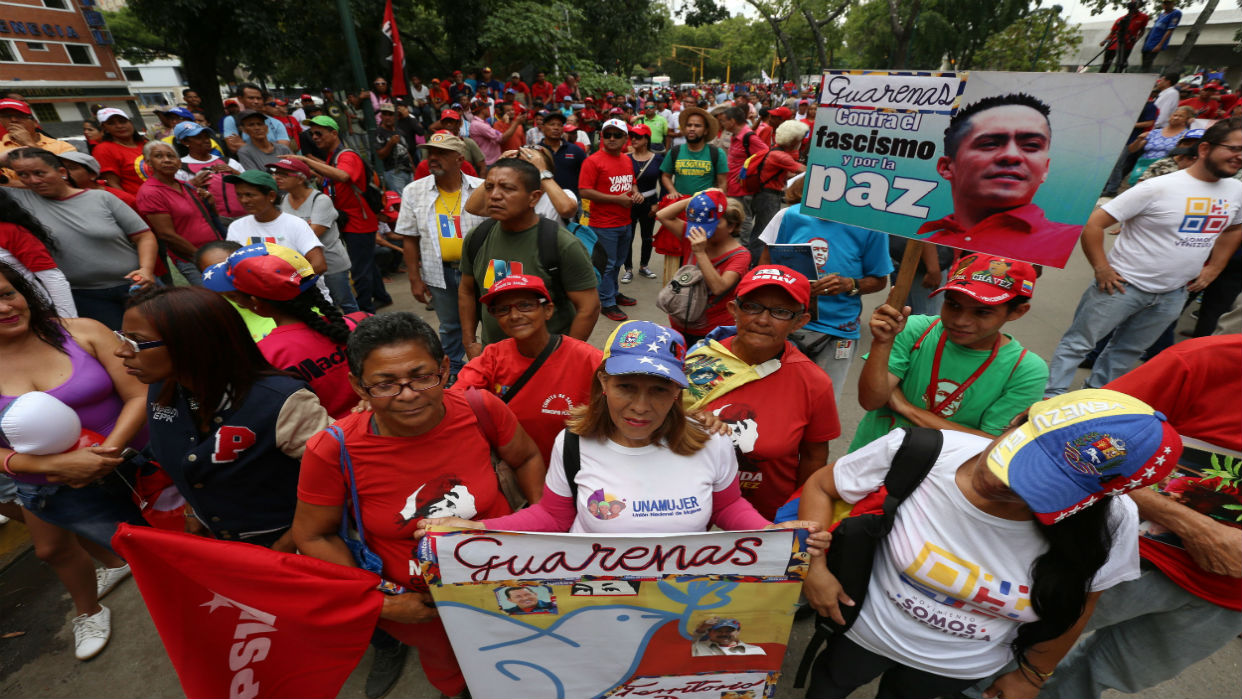
\includegraphics[width=300px]{6.jpg}%
\newline%
%
Con una marcha convocada por sectores del oficialismo este viernes rechazaron los anuncios promovidos por el gobierno de los Estados Unidos contra Venezuela.\newline%
La movilización se inició en horas del mediodía y cubrió distintas zonas de oeste de Caracas, entre ellas la avenida Los Ilustres, Nueva Granada, Roca Tarpeya, Plaza España hasta llegar al Calvario en el centro de la ciudad.%
\newline%
%
Con un mensaje por la paz repudiaron las declaraciones que expresara en días pasados,  el presidente de los Estados Unidos, Donald Trump, durante la 73º Asamblea General de la Organización de las Naciones Unidas (ONU).  Trump aseguró que "el presidente Maduro podría ser derrotado muy rápidamente si los militares deciden hacer eso".%
\newline%
%
El vicepresidente del Partido Socialista Unido de Venezuela (PSUV), Diosdado Cabello, quién encabezo la movilización junto a otros dirigentes manifestó que "Venezuela apuesta al diálogo. Nosotros podemos dialogar con quien sea, sin vender nuestros principios y traicionar nuestras creencias".%
\newline%
%
"Hemos sido objeto en los últimos cuatro años de ataques como no lo ha recibido ningún otro país, no estamos pidiendo a nadie que nos regale nada, no pretendemos un canal humanitario, estamos solicitando que nos liberen de las sanciones y del bloqueo para poder comprar las medicinas, los alimentos y todo lo necesario para el  pueblo", afirmó. Diosdado Cabello.%
\newline%
%
"El presidente de Estados Unidos está preocupado por el apoyo financiero de China y de ese grupo de países constituido también por Rusia y Bolivia por brindar su respaldo moral a Venezuela", expresó.%
\newline%
%
También informó que a alta comisionada para los Derechos Humanos de la ONU, Michelle Bachelet, "puede venir a Venezuela cuando quisiera, el país no está atravesando ninguna crisis humanitaria, sino una guerra de otros países en su contra."%
\newline%
%
El pasado 27 de septiembre, el Consejo de Derechos Humanos de la ONU aprobó una resolución sobre la crisis humanitaria, en la cual instó al Ejecutivo Nacional  a aceptar la asistencia para hacer frente a la escasez de medicamentos y alimentos, denunciada por diferentes organismos.%
\newline%
%
Congreso este fin de semana%
\newline%
%
Diosdado Cabello recordó que durante este sábado y domingo se  realizará el IV Congreso del PSUV,  en conjunto con la Juventud del Partido Socialista Unido de Venezuela, para tratar temas de organización política.%
\newline%
%
Añadió que el presidente Nicolás Maduro, solicitó que la plenaria se realice para seguir revisando los acuerdos del programa económico.\newline%
"Se ha realizado un despliegue en el territorio nacional que ha solicitado el presidente Maduro, con el tema organizativo en cada uno de los estados para seguir profundizando la organización del PSUV para atender las necesidades del pueblo", aseveró.%
\newline%
%
"Este Congreso dará resultados en todo lo que corresponde a la proyección del partido durante los próximos 4 años y en la construcción de nuevas estrategias políticas, en todo el territorio nacional con la recolección de conclusiones en los debates y asambleas que se han realizado en estos últimos meses", agregó. Cabello.%
\newline%
%
A la fecha, el PSUV ha realizado dos encuentros donde se han definido instancias de trabajo político, y el apoyo a las acciones económicas del Gobierno.%
\newline%
%
\end{document}